\documentclass[12pt]{beamer}
\usetheme[progressbar=frametitle]{metropolis}
\usepackage{appendixnumberbeamer}
\usepackage{tabularx}
\usepackage{booktabs}
\usepackage[scale=2]{ccicons}
\usepackage{pgfplots}
\usepackage{xspace}
\usepackage{bm}
\usepackage{adjustbox}
\usepackage{changepage}
\usepackage{xcolor}
\usepgfplotslibrary{dateplot}
\setbeamercovered{transparent=30,again covered={\opaqueness<1->{30}}}

\title{Optimal Database Design Problem}
\author{Defended by: Group 06 \texorpdfstring{\\Magnani, Marchi, Moncada, Iaia,}{}\texorpdfstring{\\Palmieri, Ondesca, Ombe}{}}
\date{9, January 2019}
\institute{Politecnico di Torino\\Optimization Methods and Algorithms}

\begin{document}
  \maketitle
  \section{Algorithm presentation}
  % ------------------------------------------------------------------------------------------------------------
  %													Algorithm presentation
  % ------------------------------------------------------------------------------------------------------------
  {
  \usebackgroundtemplate{
\includegraphics[width=\paperwidth]{res/Genetic}}
  \color{white}
  \begin{frame}[fragile]{Genetic Algorithm}
    \begin{center}
      {\fontsize{30}{40}\selectfont \textbf{Why?}}
    \end{center}
  \end{frame}
  }

  \begin{frame}[fragile]{Main Features}
    \begin{columns}
      \begin{column}{0.5\textwidth}
        Key points of our implementation:
        \begin{itemize}
          \item<1> Scalability and adaptability
          \item<2> Multistart and restart
          \item<3> Multithreading
          \item<4> Large Solution Space exploration
        \end{itemize}
      \end{column}
      \begin{column}{0.5\textwidth}
          \only<1>{
            
\includegraphics[scale=0.2]{res/Scalability}
          }
          \only<2>{
            
\includegraphics[scale=0.18]{res/Restart}
          }
          \only<3>{
            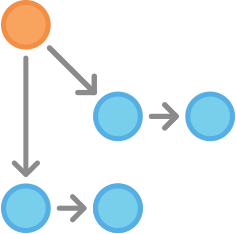
\includegraphics[scale=0.6]{res/Multithreading}
          }
          \only<4>{
            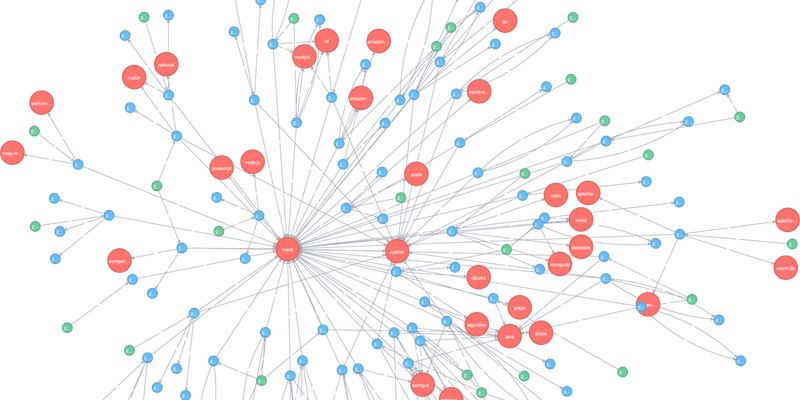
\includegraphics[scale=0.8]{res/SolutionSpace}
          }
      \end{column}
    \end{columns}
  \end{frame}

  \begin{frame}[fragile]{Solution Set Selection procedures}
    \begin{columns}
      \begin{column}{0.5\textwidth}
        Solution Set Selection procedures implemented:
        \begin{itemize}
          \item<1> Roulette
          \item<2> Tournament
          \item<3> Random
        \end{itemize}
      \end{column}
      \begin{column}{0.5\textwidth}
          \only<1>{
            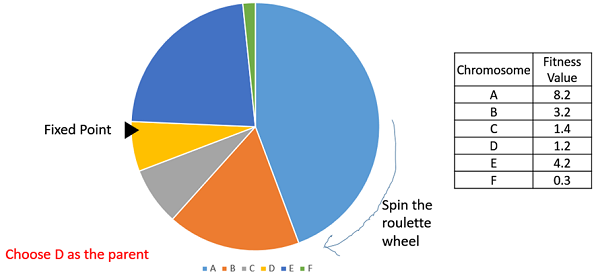
\includegraphics[scale=1.0]{res/Roulette}
          }
          \only<2>{
            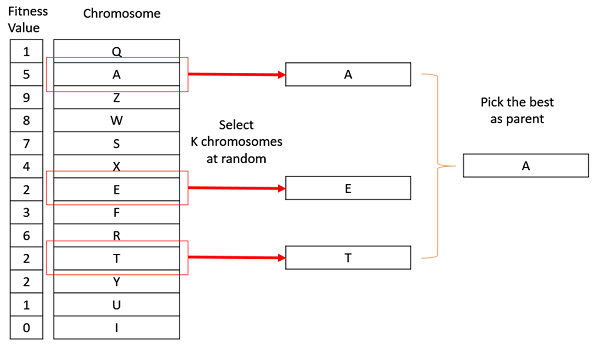
\includegraphics[scale=1.0]{res/Tournament}
          }
          \only<3>{
            
\includegraphics[scale=0.15]{res/Random}
          }
      \end{column}
    \end{columns}
  \end{frame}

  \begin{frame}[fragile]{Children generation methods}
    Children generation methods implemented:
    \begin{itemize}
      \item Mutation
      \begin{itemize}
        \item 2-bit instead of 1
        \item 70\% chance to be chosen
      \end{itemize}
      \item Inversion
      \begin{itemize}
        \item traditional approach adapted to the instance dimension
        \item 15\% chance to be chosen
      \end{itemize}
      \item Crossover
       \begin{itemize}
        \item traditional approach
        \item 15\% chance to be chosen
      \end{itemize}
    \end{itemize}
  \end{frame}

  \begin{frame}[fragile]{Children generation methods}
    An our 'local search' is enhanced by replacing all the non-parent elements (which are supposed to be the worst ones) with the actual best solution.\\
    \begin{center}
      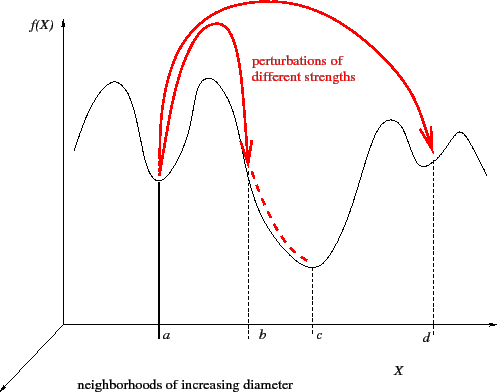
\includegraphics[scale=0.3]{res/LocalSearch}
    \end{center}
  \end{frame}

  \begin{frame}[fragile]{Algorithm steps}
    \begin{adjustwidth}{-2em}{-2em}
      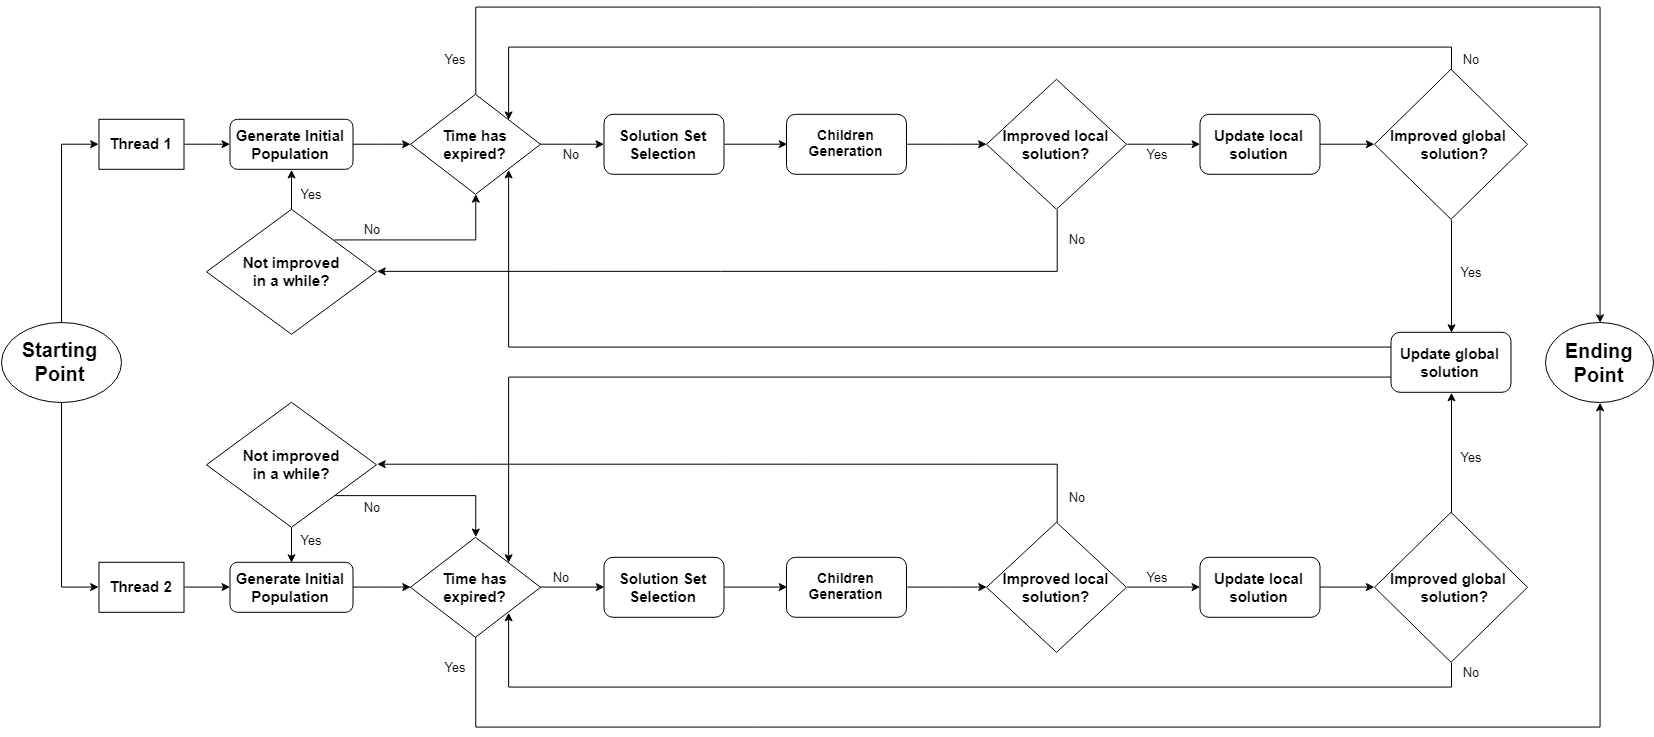
\includegraphics[scale=0.21]{res/Algorithm}
    \end{adjustwidth}
  \end{frame}

  \section{Results analysis}
  % ------------------------------------------------------------------------------------------------------------
  %													Results
  % ------------------------------------------------------------------------------------------------------------
  \begin{frame}[fragile]{Result Analysis}
    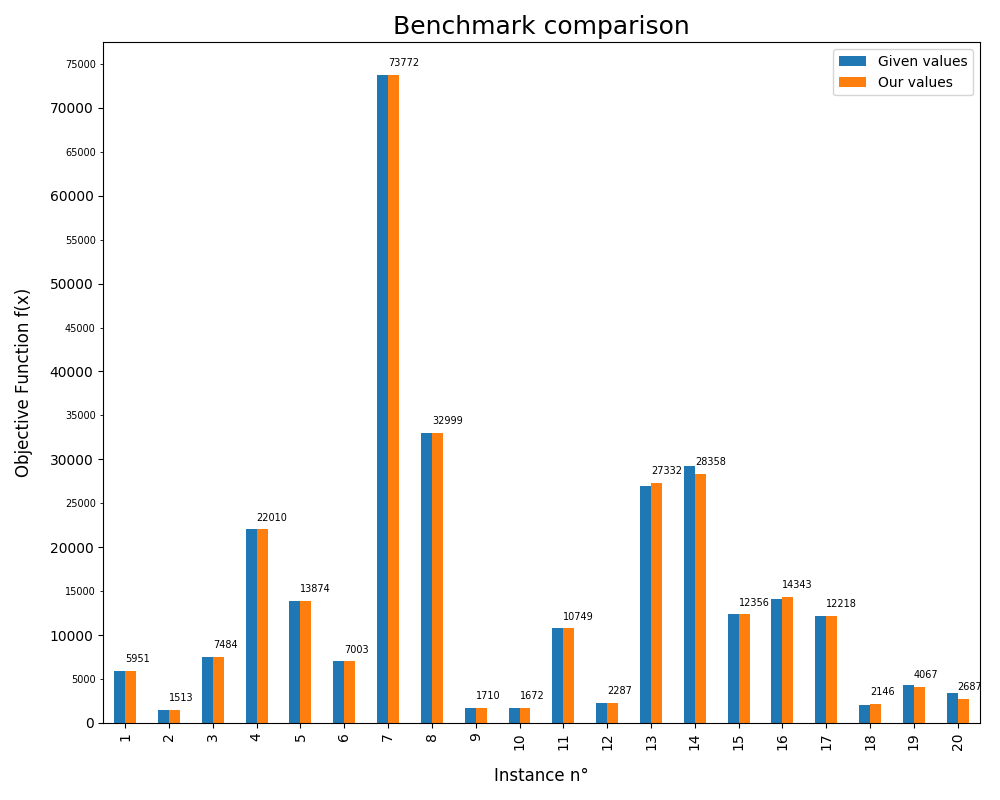
\includegraphics[scale=0.4]{res/benchmarkComparison}
  \end{frame}

    \begin{frame}[fragile]{Benchmark Comparison}
    \adjustbox{max width=0.8\textwidth}{%
    \begin{columns}
      \begin{column}{0.8\textwidth}
        \footnotesize
        \begin{tabular}{|c|c|c||c|} 
          \hline
          \textbf{Instance} & \textbf{Given Results} & \textbf{Our Results} & \textbf{Gap(\%)} \\
          \hline
          instance01 & 5951 & 5951 & 0 \\
          instance02 & 1513 & 1513 & 0 \\
          instance03 & 7484 & 7484 & 0 \\
          instance04 & 22010 & 22010 & 0 \\
          instance05 & 13874& 13874 & 0 \\
          instance06 & 7003 & 7003 & 0 \\
          instance07 & 73772 & 73772 & 0 \\
          instance08 & 32999 & 32999 & 0 \\
          instance09 & 1710 & 1710 & 0 \\
          instance10 & 1672 & 1672 & 0 \\
          instance11 & 10749 & 10749 & 0 \\
          instance12 & 2287 & 2287 & 0 \\
          \hline
          instance13 & 26938 & 27332 & -1.46 \\
          instance14 & 29280 & 28358 & 3.15 \\
          instance15 & 12351 & 12356 & -0.04 \\
          instance16 & 14110 & 14343 & -1.65 \\
          instance17 & 12218 & 12218 & 0 \\
          instance18 & 2081 & 2146 & \color{green}-3.12 \\
          instance19 & 4257 & 4067 & 4.46 \\
          instance20 & 3406 & 2687 & \color{red}21.11 \\
          \hline
        \end{tabular}
      \end{column}
      \begin{column}{0.2\textwidth}
        \footnotesize
        \begin{tabular}{|c|c|} 
          \hline
           & \textbf{Gap(\%)}\\
          \hline
          Best & \color{green} -3.12 \\
          Worst & \color{red} 21.11 \\
          Avg & 1.12\\
          \hline
        \end{tabular}
      \end{column}
    \end{columns}
    }
  \end{frame}

  \begin{frame}[fragile]{Result Analysis}
    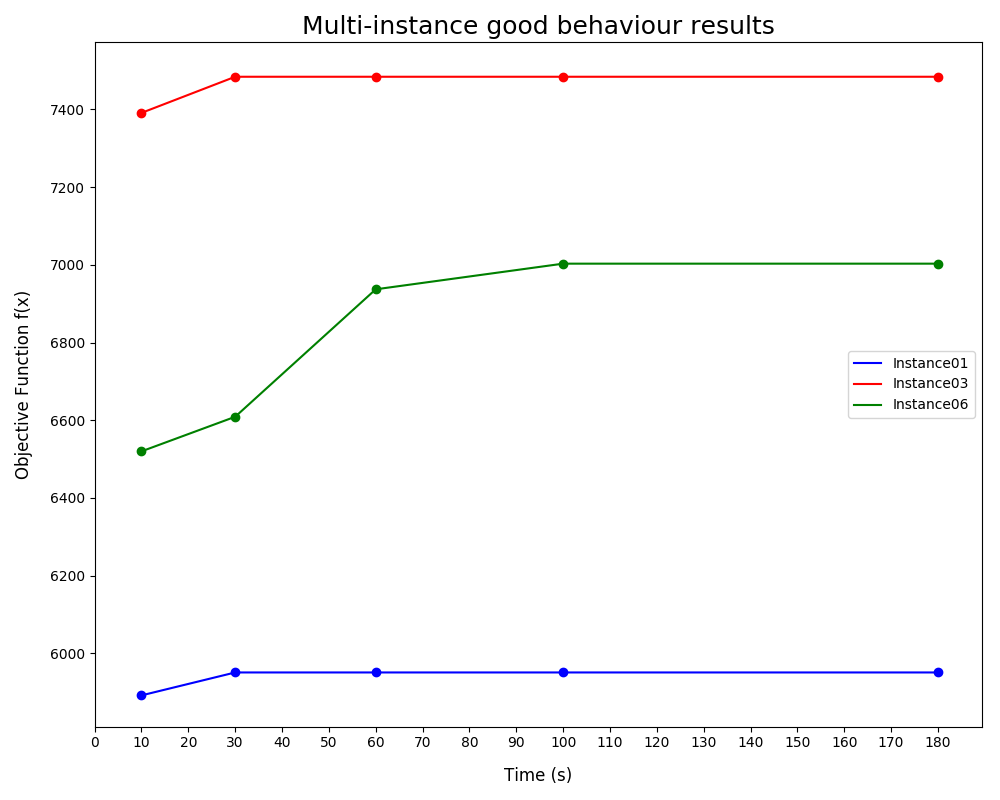
\includegraphics[scale=0.4]{res/goodInstances}
  \end{frame}

  \begin{frame}[fragile]{Result Analysis}
    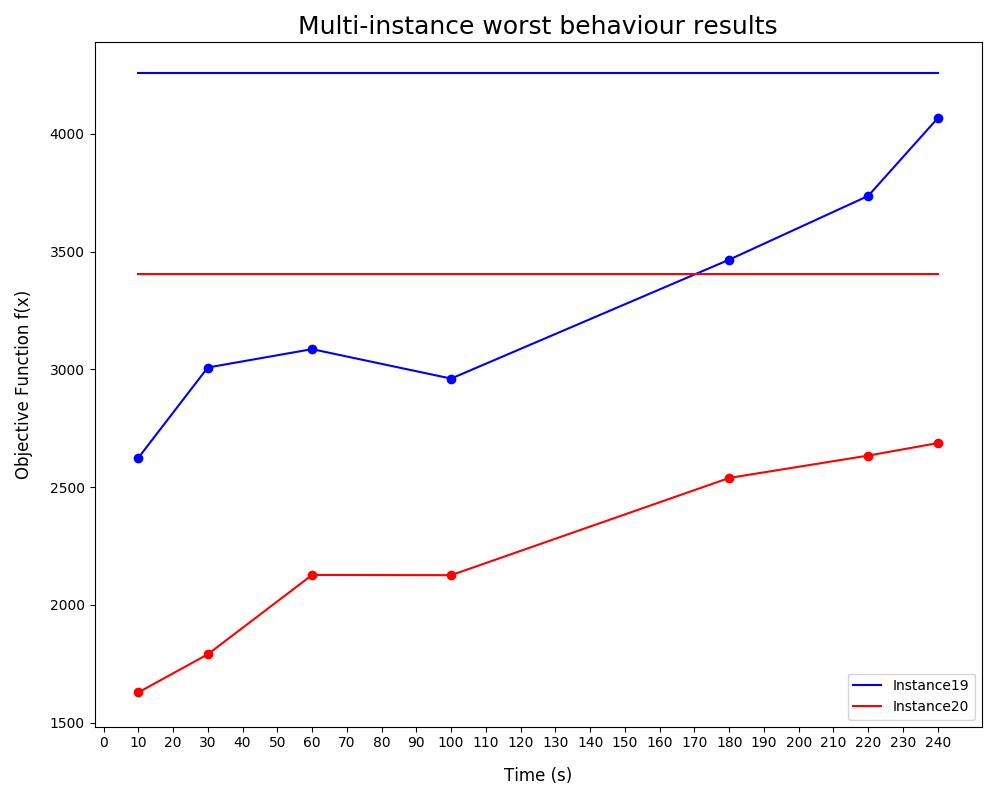
\includegraphics[scale=0.4]{res/badInstances}
  \end{frame}

  \begin{frame}[fragile]{Result Analysis}
    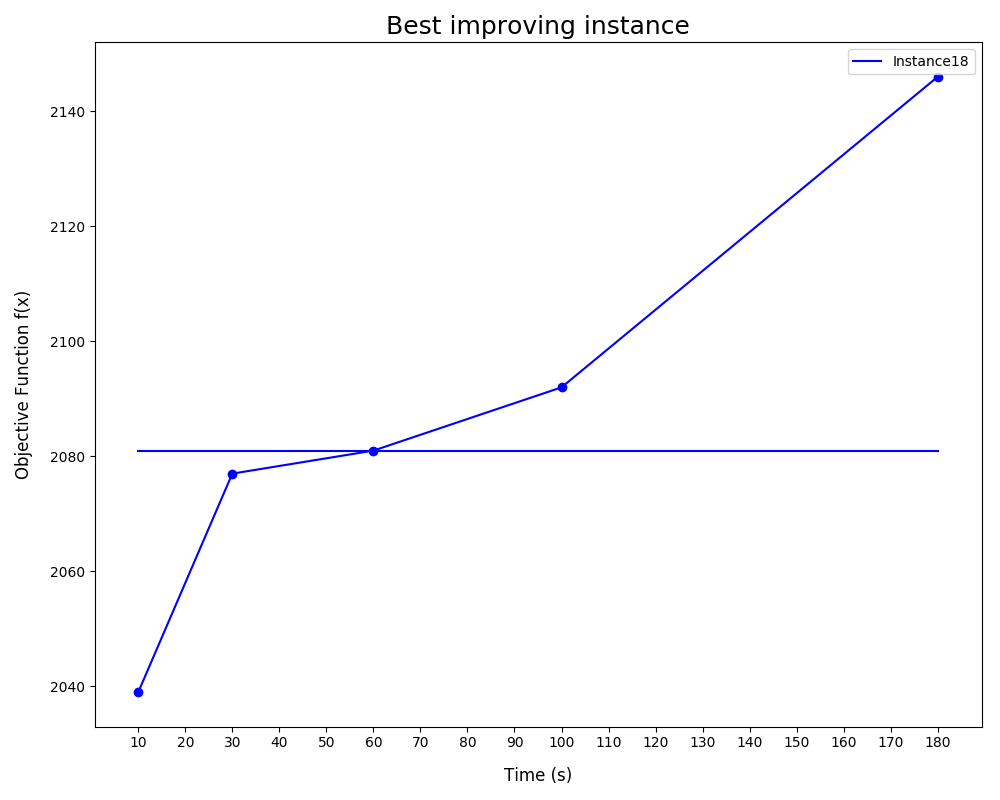
\includegraphics[scale=0.4]{res/bestImproving}
  \end{frame}

  \begin{frame}[fragile]{Result Analysis}
    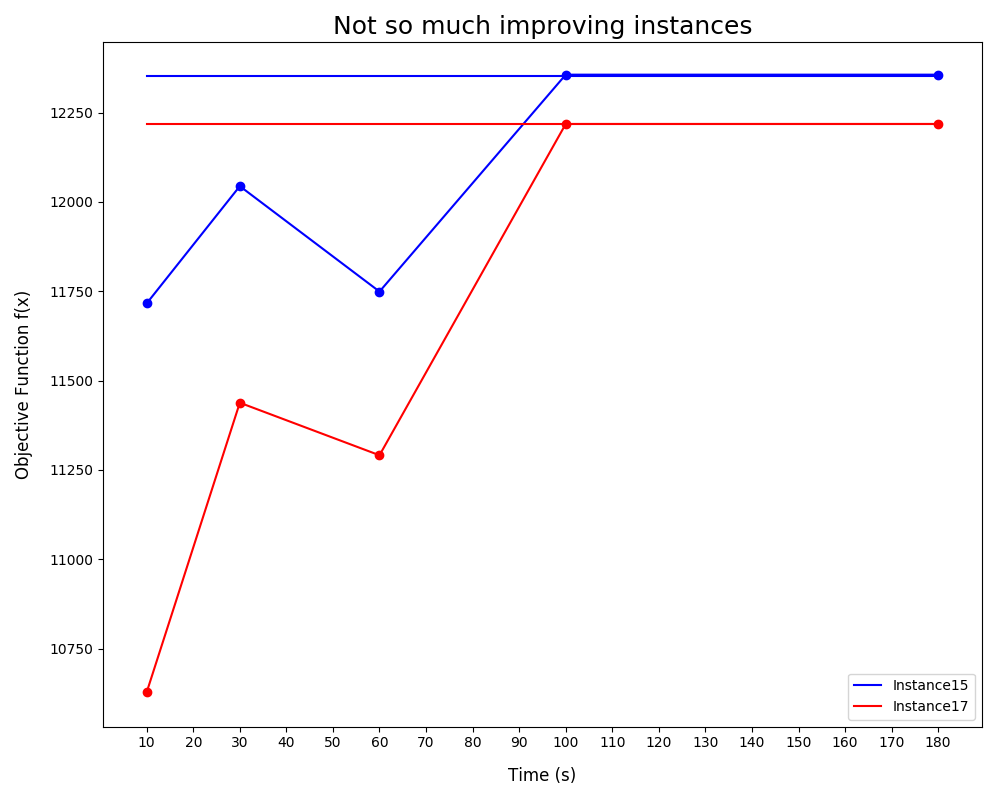
\includegraphics[scale=0.4]{res/notMuchImproving}
  \end{frame}

  % ------------------------------------------------------------------------------------------------------------
  %													End
  % ------------------------------------------------------------------------------------------------------------
  \begin{frame}[standout]
  	THE END
  \end{frame}

\end{document}